\documentclass[11pt]{article}
\usepackage[utf8]{inputenc}

\title{Generative Adversarial Networks}
\author{Jacob Smith}
\date{December 12, 2017}

\usepackage{natbib}
\usepackage{graphicx}

\usepackage{parskip}

\graphicspath{{./img/}}

\begin{document}
\maketitle

\begin{abstract}
    General Adversarial Networks have
\end{abstract}

\section{Introduction}
Deep learning have made astounding progress within the past decade. Discriminative models have recently surpassed the abilities of human within the domain of pattern recognition \citep{2014arXiv1404.7828S}. These successes can attributed to vast, high dimension datasets in conjunction with large neural networks using linear activation functions, dropout regularization techniques and backpropagation to update the parameters \citep{2014arXiv1406.2661G}. However, deep learning possesses many more ambitious goals. Until recently, success has mostly been seen with supervised classifiers; however, deep generative models now competitively rival their discriminative counterparts.

Generative models learn the joint probability distribution $p(x,y)$ of an input $x$ and label $y$ whereas discriminative models directly learn the conditional probability $p(y|x)$. Generative models may be used as classifiers using Bayes rules to calculate the conditional probability $p(x,y)$ which can then be used to make predictions \citep{NIPS2001_2020}. Depending on the model, knowledge of the probability distribution can be created both explicitly and implicitly \citep{Goodfellow-et-al-2016}. Those which do not directly model a probability distribution offer mechanisms which require implicit knowledge of the underlying distribution, such as creating a sample from that distribution \citep{Goodfellow-et-al-2016}. As humans, we are able to understand the world around us with tremendous precision. It is easy to underestimate the complexity of the data we process to accomplish this feat. Although progress within the machine learning field is rapidly advancing, computers still have limited understanding of the data the process. Generative models, especially deep generative models, offer promising results towards this goal \citep{genmodelingopenai}.

\begin{figure}
\centering
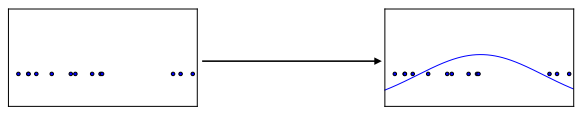
\includegraphics[scale=0.7]{pdf}
\caption{The process density estimation of one-dimensional data and a Gaussian distribution \citep{2017arXiv170100160G}. Generative models take a dataset $D$, sourced from a distribution $p_{data}$, a create an estimate of that distribution $p_{model}$.}
\label{fig:pdf}
\end{figure}

The process of training a generative model is very similar to a discriminative model. Using large amounts of data collected from a specific domain, we train the model to generate data from that domain. As these models have fewer parameters than that the number of data samples, they are forced to internalize some representation of the data. Although, unlike supervised training, there exists no explicit desired output. The problem becomes defining a cost function which forces the generative model to produce data more like that of the domain.

Generative adversarial networks (GANs), first introduced in 2014, offer a new framework for estimating generative models with use of an adversarial process \citep{2014arXiv1406.2661G}. These models offer a clever approach to solving the aforementioned problem of explicitly defining a cost function. Rather than training a single model, a discriminator is introduced. These two networks are pitted against each other in a minimax game. The generative model $G$ attempts to produce data that resembles that of the training set while the discriminative model $D$ attempts to classify whether or not a sample was real of generated. To train this network, $G$ attempts to maximize the error rate of $D$ whereas $D$ attempts to minimize it. Backpropagation is used to update the parameters and to train each model. In the ideal case, $D$ is unable to distinguish the generated samples from the real samples and produces an error rate of $\frac{1}{2}$ \citep{2014arXiv1406.2661G}.



\section{Conclusion}
Generative models are currently being applied to many problems \citep{genmodelingopenai}; however, they offer many more possibilities due to their ability to understand the data they are given.

\bibliographystyle{plain}
\bibliography{references}
\end{document}
